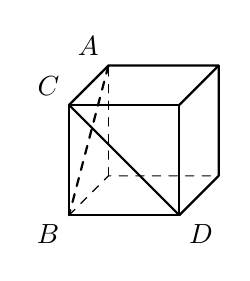
\begin{tikzpicture}[>=latex, scale=1.0, line join=round, line cap=round]
  % Cube vertices
  \coordinate (FBL) at (0, 0);
  \coordinate (FBR) at (1.4, 0);
  \coordinate (FTR) at (1.4, 1.4);
  \coordinate (FTL) at (0, 1.4);

  \coordinate (BBL) at (0.5, 0.5);
  \coordinate (BBR) at (1.9, 0.5);
  \coordinate (BTR) at (1.9, 1.9);
  \coordinate (BTL) at (0.5, 1.9);

  % Dashed cube edges
  \draw[dashed, thin] (FBL) -- (BBL) -- (BBR);
  \draw[dashed, thin] (BBL) -- (BTL);

  % Solid cube edges
  \draw[thick] (FBL) -- (FBR) -- (FTR) -- (FTL) -- cycle;
  \draw[thick] (FTL) -- (BTL) -- (BTR) -- (FTR);
  \draw[thick] (BTR) -- (BBR) -- (FBR);

  % Problem lines: AB dashed, CD solid
  \draw[dashed, thick] (BTL) -- (FBL);
  \draw[thick] (FTL) -- (FBR);

  % Labels
  \node[above left] at (BTL) {$A$};
  \node[below left] at (FBL) {$B$};
  \node[above left] at (FTL) {$C$};
  \node[below right] at (FBR) {$D$};
\end{tikzpicture}
